\section{Design}
\subsection{Design Overview}
This design section is split into a number of sections. Firstly I detail the choices for the various hardware components based on the outcome of the results of the research section above, then I move on to the two software components that make up the overall system. We start with the Honeypot application that finds and attacks vulnerable devices, and then move on to looking at the structure of the leaky Android application and how to overcome the problem of using platform specific code within the game. 
\subsection{Overall System Architecture}
The scenario that this project hypothetically aims to work in is in an area with high traffic, such as a Student Union bar, or a busy public transport station. In reality the applications are designed to meet the ethical guidelines set forth at the beginning of the project whereby a user's consent must be gained prior to taking place in any experimentation. Due to this restriction care must be taken within the design to ensure, where appropriate, devices are filtered and ignored on a set of criteria. This criteria may be MAC address of devices broadcasting probe requests or the SSID present in probe requests. As set out in the requirements the filter will be based on the latter of the two proposed, filtering devices based on the SSID they are probing for. In doing so removes the limitation of testing one device at a time- theoretically having to update the MAC address filter for each new device- and allows us to connect multiple devices running different operating systems at the same time to determine the effectiveness of the overall implementation of the honeypot attack. It should be noted that the leaky application, designed to demonstrate the ease in which applications can broadcast personal data unencrypted, will only be available on Android due to the relative simplicity in creating an application for the environment, and availability of devices. 

\begin{figure}[h!]
\centering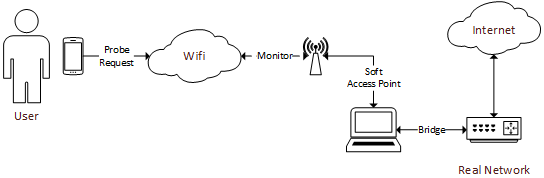
\includegraphics[width=\linewidth]{design/figures/overall.png}
\caption{Overall system architecture- may need to change.}
\end{figure}

A soft access point is created on the detection of a valid probe request, which is defined as being a request from a device that is looking to reconnect to a network with no authentication method, and the network traffic is then bridged to an actual network to ensure that the user is still able to access the internet, and the attacker can monitor passing traffic.

\subsection{Honeypot}
\subsubsection{High Level Program Flow}
Figure \ref{fig:honeypot_flow} details the application flow for the honeypot application. 

\begin{figure}[h!]
\centering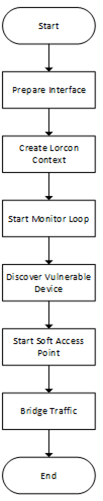
\includegraphics{design/figures/honeypot-flow.png}
\caption{Overall system architecture- may need to change.}
\label{fig:honeypot_flow}
\end{figure}

\subsubsection{Discovering Vulnerable Devices}
Figure \ref{fig:discover_device_seq} details the process in which the application goes through to discover a vulnerable device. It parses frame types until it finds a probe request, then sending a response to trigger an association request from the device so it can determine the authentication type that the previous access point used. If it was an open access point that the device had previously connected to it returns a success value and allows the application to move on to the next  stage of the attack, creating the fake access point.

\begin{figure}[h!]
\centering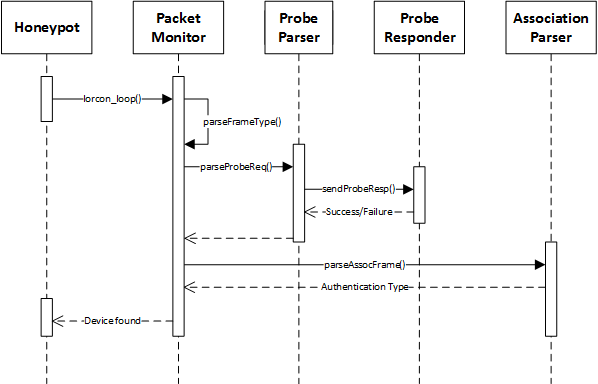
\includegraphics[width=\linewidth]{design/figures/discover-device-seq.png}
\caption{Discovering vulnerable device sequence diagram.}
\label{fig:discover_device_seq}
\end{figure}
\clearpage
\subsection{Android Game}
The Android game design is relatively simple. It consists of two classes that inherit from the libgdx screen class, with the GameScreen class holding the GameRenderer and GameWorld which renders and holds the game state respectively doing the majority of the work.

\begin{figure}[h!]
\centering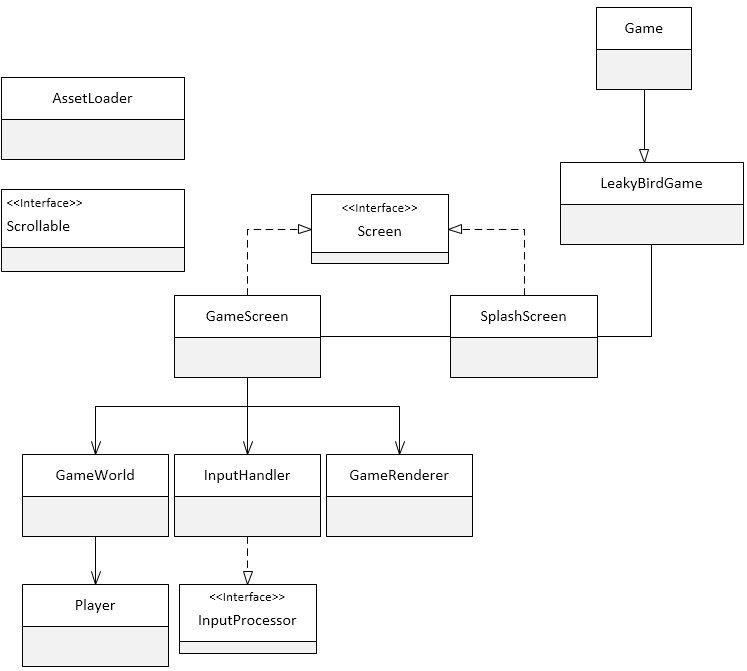
\includegraphics[width=\linewidth]{design/figures/ag-cd.png}
\caption{Android game class diagram.}
\end{figure}
\clearpage
\subsubsection{Android Location Provider}
To successfully use platform specific functionality within the libgdx game environment an interface needs to be created to allow use of the functions. More detail on this can be found in the implementation section; however, below details the classes required to provide the game with the ability to get location information from the Android device.

\begin{figure}[h!]
\centering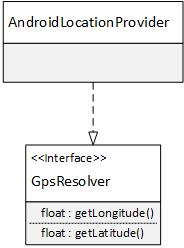
\includegraphics{design/figures/ag-lp-cd.png}
\caption{Android game libgdx location interface.}
\end{figure}

\subsubsection{TCP Client Provider}
Android applications require any network communications to be performed on a separate thread to that which the UI is currently running on. This stops the application from becoming unresponsive during long connection times or heavy data transfers. As a result of this the TCP client connection, data transfer, and disconnection must run on an AsyncTask when executed otherwise the application will throw an android.os.NetworkOnMainThreadException, so this requires another interface to be written to encapsulate the Android specific library. 
\clearpage
\begin{figure}[h!]
\centering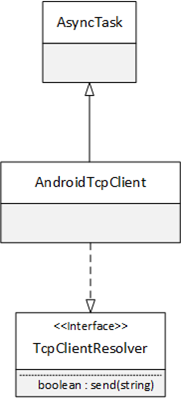
\includegraphics{design/figures/tcp-cd.png}
\caption{Android TCP client class diagram.}
\end{figure}

Similar to the GpsResolver class, the Android MainActivity will pass through an AndroidTcpClient that implements the TcpClientResolver interface for the game to make of use of when it needs to transmit data to to the server.

\begin{figure}[h!]
\centering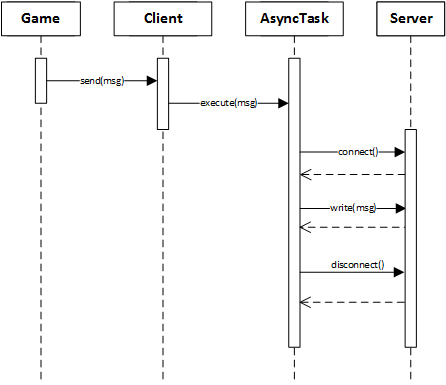
\includegraphics[width=\linewidth]{design/figures/tcp-client-sd.png}
\caption{Android TCP client sequence diagram.}
\end{figure}

The interface exposes the send function to the application to allow it to send data by internally using a class that extends AsyncTask.

\subsubsection{TCP Message Structure}
\label{design:tcp-structure}
Due to this application leaking data by design, the message protocol does not require any encryption and can be relatively simple. There is only one type of message the application needs to send- data. The packet needs to include a uniquely identifiable value for the device that is running the game in order to track users. As it has relatively simple requirements the packet structure will be the packet type, device unique identifier followed by the payload. The fields will be delimited by a comma to allow the server to tokenize the packet for processing.
%%%%%%%%%%%%%%%%%%%%%%%%%%%%%%%%%%%%
\clearpage